\documentclass[sigconf]{acmart}

\usepackage{booktabs} % For formal tables
\usepackage{todonotes}

% Our added packages
\usepackage[ruled]{algorithm2e}
\usepackage{tabu}

%\usepackage{algorithm}
%\usepackage{algorithmic}

\renewcommand{\baselinestretch}{0.93} 


% Copyright
%\setcopyright{none}
%\setcopyright{acmcopyright}
%\setcopyright{acmlicensed}
%\setcopyright{rightsretained}
%\setcopyright{usgov}
%\setcopyright{usgovmixed}
%\setcopyright{cagov}
%\setcopyright{cagovmixed}

\copyrightyear{2017} 
\acmYear{2017} 
\setcopyright{rightsretained} 
\acmConference{GECCO '17 Companion}{July 15-19, 2017}{Berlin, Germany}
\acmDOI{http://dx.doi.org/10.1145/3067695.3075617}
\acmISBN{978-1-4503-4939-0/17/07}

\begin{document}

\title{Visualizing genetic programming ancestries using graph databases}

\author{Nicholas Freitag McPhee}
\orcid{0000-0002-6495-2612}
\affiliation{%
	\institution{University of Minnesota, Morris}
	% \streetaddress{600 E. 4th Street}
	\city{Morris} 
	\state{Minnesota} 
	\country{USA}
}
\email{mcphee@morris.umn.edu}

\author{Maggie M. Casale}
\affiliation{
	\institution{Design Center Inc.}
	\city{St. Paul}
	\state{Minnesota}
	\country{USA}
}
\email{mcasale@designcenterideas.com}

\author{Thomas Helmuth}
\orcid{0000-0002-2330-6809}
\affiliation{%
	\institution{Washington and Lee University}
	\city{Lexington} 
	\state{Virginia} 
	\country{USA}
}
\email{helmutht@wlu.edu}

\author{Lee Spector}
\orcid{0000-0001-5299-4797}
\affiliation{%
	\institution{Hampshire College}
	\city{Amherst}
	\state{Massachusetts}
	\country{USA}
}
\email{lspector@hampshire.edu}

\begin{abstract}

Previous work has demonstrated the utility of graph databases as a tool for collecting and analyzing ancestry in evolutionary computation runs. That work focused on sections of individual runs, whereas this poster illustrates the application of these ideas on the entirety of large runs (up to one million individuals) and combinations of multiple runs.
Here we use these tools to generate graphs showing \emph{all} the ancestors of successful individuals from a variety of stack-based genetic programming runs on software synthesis problems. These graphs highlight important moments in the evolutionary process. They also allow us to compare the dynamics when using different evolutionary tools, such as different selection mechanisms or representations, as well as comparing the dynamics for successful and unsuccessful runs.

\end{abstract}

\begin{CCSXML}
	<ccs2012>
	<concept>
	<concept_id>10003120.10003145.10003146.10010892</concept_id>
	<concept_desc>Human-centered computing~Graph drawings</concept_desc>
	<concept_significance>500</concept_significance>
	</concept>
	<concept>
	<concept_id>10003120.10003145.10003147.10010364</concept_id>
	<concept_desc>Human-centered computing~Scientific visualization</concept_desc>
	<concept_significance>500</concept_significance>
	</concept>
	<concept>
	<concept_id>10010147.10010178.10010205.10010206</concept_id>
	<concept_desc>Computing methodologies~Heuristic function construction</concept_desc>
	<concept_significance>300</concept_significance>
	</concept>
	<concept>
	<concept_id>10010147.10010257.10010293.10011809.10011813</concept_id>
	<concept_desc>Computing methodologies~Genetic programming</concept_desc>
	<concept_significance>300</concept_significance>
	</concept>
	</ccs2012>
\end{CCSXML}

\ccsdesc[500]{Human-centered computing~Graph drawings}
\ccsdesc[500]{Human-centered computing~Scientific visualization}
\ccsdesc[300]{Computing methodologies~Heuristic function construction}
\ccsdesc[300]{Computing methodologies~Genetic programming}

\keywords{visualization; genetic programming; graph database; ancestry}

\maketitle

\section{Introduction}
\label{sec:introduction}

Reporting results of genetic programming (GP) and evolutionary computation is frequently limited to aggregate statistics such as mean best fitness or percentage of successful runs. Unfortunately this fails to convey the complex dynamics of such evolutionary systems and obscures or omits potentially valuable information about \emph{why} the runs behaved as they did. Previous work~\cite{McPhee:2015:GPTP} has demonstrated the utility of graph databases as tools for collecting and analyzing ancestry in GP runs, but was focused on sections of individual runs.

In this poster we illustrate the use of these tools as a means of exploring entire ancestry trees. We use the Titan graph database\footnote{\url{http://thinkaurelius.github.io/titan/}} along with the Gremlin shell and the Tinkerpop query tools\footnote{\url{https://tinkerpop.incubator.apache.org/}} to store the parent-child relationships from genetic programming runs, and to extract the ancestry trees of specified individuals. We then visualize these subgraphs using the Graphviz \texttt{dot} graph layout tool\footnote{\url{http://www.graphviz.org/}}.

\section{Example: Success vs. failure}
\label{sec:examples}

Here we illustrate these ideas by extracting and plotting the ancestors of final generation individuals in both a successful (Figure~\ref{fig:success}) and an unsuccessful run (Figure~\ref{fig:fail}) of the replace-space-with-newline software synthesis problem~\cite{Helmuth:2015:GECCO,Helmuth:2015:dissertation} using lexicase selection~\cite{Helmuth:2014:ieeeTEC}. The successful run shows all the ancestors of that run's winners (i.e., individuals with total error 0, discovered at generation 129). The unsuccessful run shows the ancestors of all individuals from generation 300, when the run was terminated.

\begin{figure}[t]
	\centering
	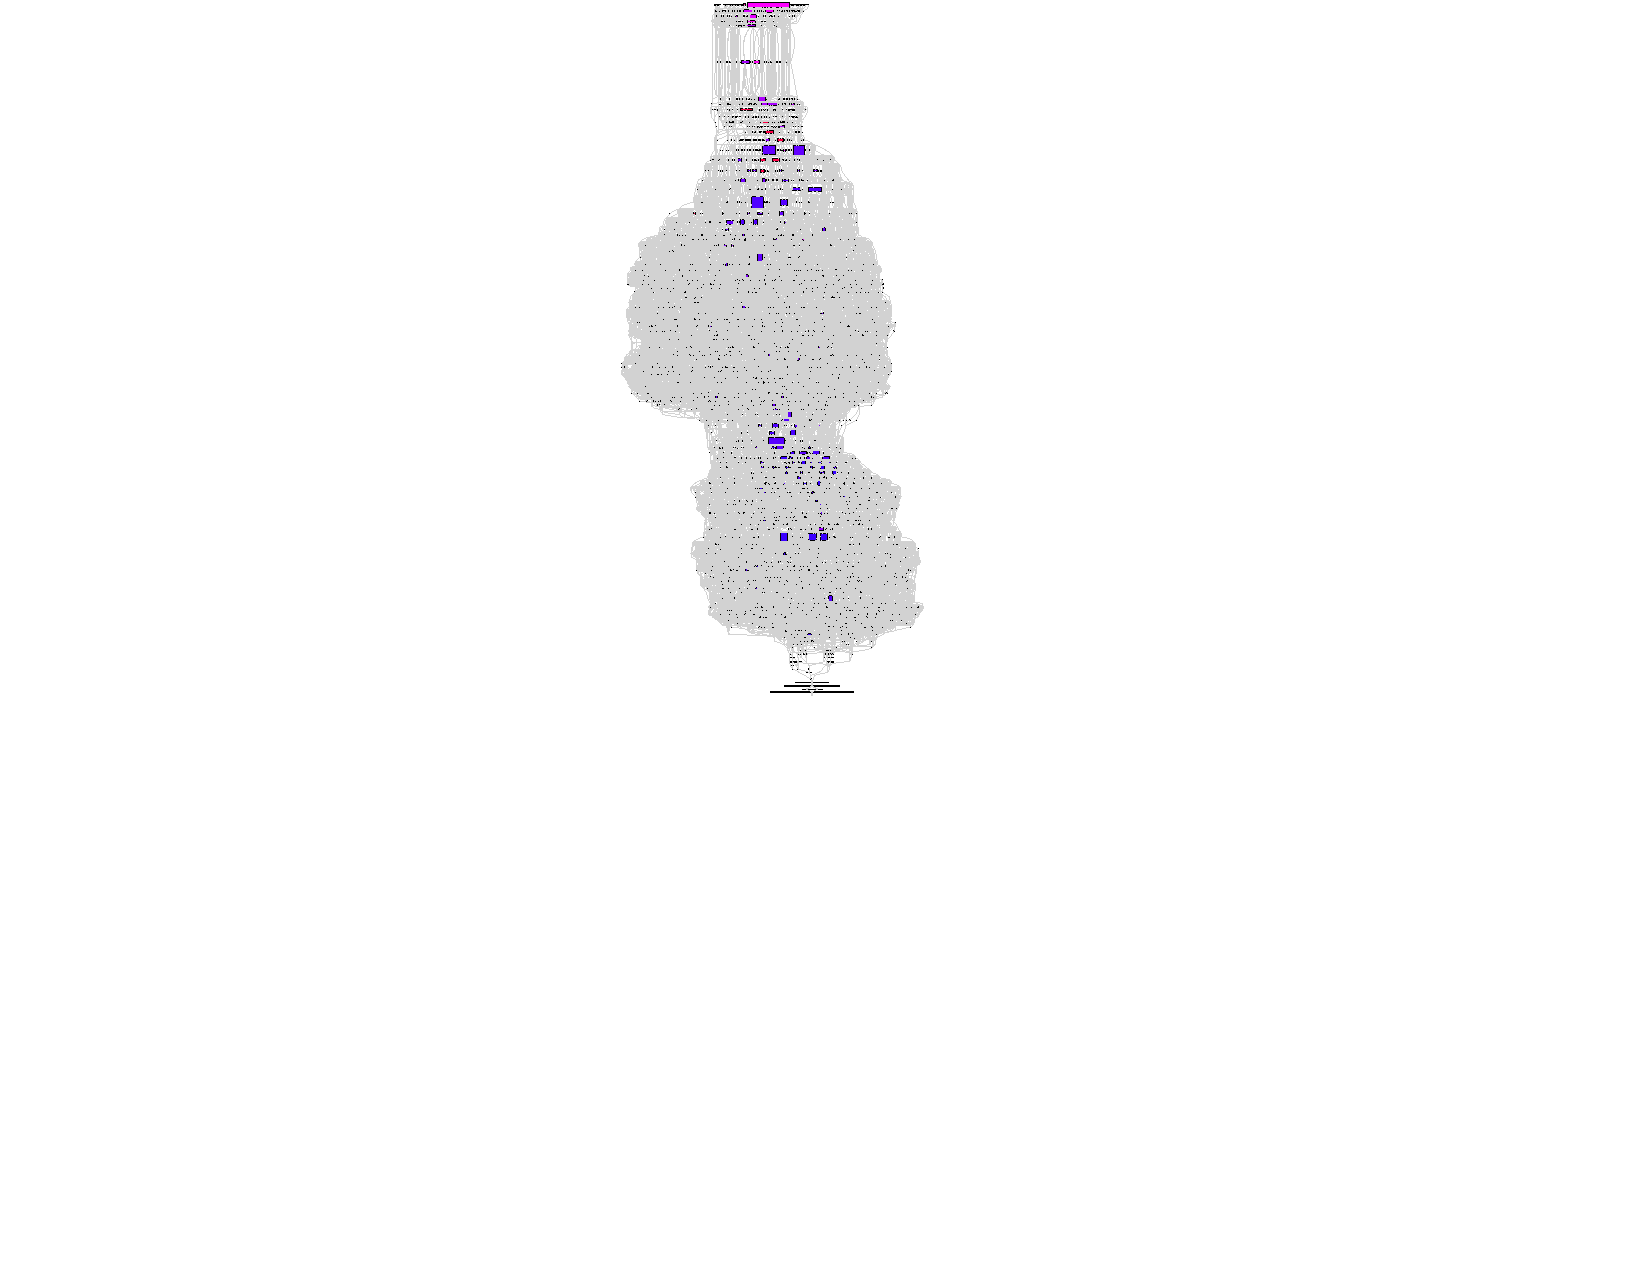
\includegraphics[height=0.5 \textheight]{../Figures/output_success.pdf}
	\caption{Ancestry tree for the one individual with total error 0 in a successful run of the replace-space-with-newline problem using lexicase selection.}
	\label{fig:success}
\end{figure}

\begin{figure}[p]
	\centering
	\includegraphics[height=0.91\textheight]{../Figures/output_fail.pdf}
	\caption{Ancestry tree for all of the individuals in the final generation for an unsuccessful run of the replace-space-with-newline problem using lexicase selection.}
	\label{fig:fail}
\end{figure}

In these figures, generations run from the initial random population at the top to the final generation at the bottom, one generation per row. Both of these runs used a population size of 1,000, but far fewer individuals are included in the graphs because only a (sometimes small) subset of the individuals in any given generation go on to be ancestors of individuals in subsequent generations. Each individual is represented as a rectangle whose width is proportional to the number of parent selections that individual received, and whose height is proportional to the number of its offspring that are included in the ancestry graph. 
% The ratio of width to number of selections is $\sfrac{1}{5}$ the ratio of height to number of ancestral children to keep the graph from getting too wide.
The color of an individual is determined by its total error; 0 total error is bright green, moving through blues to bright red, which represents total error of 10,000 or greater. A directed edge in the graph indicates a parent-child relation, with the edge going from the parent down to the child. A child with only a single incoming edge is the result of a mutation operator and children with two incoming edges are the result of a recombination; see~\cite{Helmuth:2015:dissertation,Spector:2013:GPTP} for additional details.

Both Figures~\ref{fig:success} and~\ref{fig:fail} illustrate a common pattern in the early generations where there is a substantial number of highly selected individuals (i.e., very wide rectangles). This is presumably because most individuals in the early generations perform poorly, as evidenced by the prevalence of red and pink, leaving a handful of slightly-less-bad individuals to receive the bulk of the selections. After several generations, however, the population gains competence (as evidenced by more purple and dark blue) and there are fewer instances where a single individual receives a very high proportion of the selection events, as evidenced by the large number of small rectangles.

After that initial phase, the behavior in the unsuccessful run (Figure~\ref{fig:fail}) becomes static, with the width of the graph (essentially the number of parents in each generation) remaining roughly constant, with no highly selected (i.e., wide) individuals. The colors also indicate that the total error is not improving substantially over time, remaining mostly between pink and purple. The best total error in fact remains at 234 from generation 16 to 270, although there is a gradual improvement in the last 30 generations with the best error at the end of the run being 215.

In the successful run (Figure~\ref{fig:success}), however, there are clear changes in the dynamics over time. By generation 14, the best individual is able to correctly solve 124 of the 200 test cases for replace-space-with-newline. Then starting around generation 59 there is a ``narrowing'' of the graph, with several highly selected (i.e., wide) individuals dominating the ancestry for the next ten generations. This narrowing represents an important ``discovery'' which leads to individuals that have zero error on an additional 9\% (18) of the test cases. The graph then widens out again until the rapid convergence on the solution in the final generations. The graph also highlights three highly selected individuals in generation 87 where for the first time the best individual has zero error on an additional 18 test cases.


\bibliographystyle{ACM-Reference-Format}
\bibliography{GECCO_2017_poster} 

\end{document}